\documentclass{beamer}
\usetheme{Copenhagen}
\usepackage{xeCJK}
\usepackage{pgfplots} 
\setCJKmainfont{Noto Serif CJK SC}
\setCJKmonofont{Noto Sans Mono CJK SC}
\renewcommand{\today}{\number\year 年 \number\month 月 \number\day 日}
 
 
%Information to be included in the title page:
\title{多线程并行 InSAR 数据处理\\程序的设计与实现}
\author{崔灏 PB13007103}
\institute{中国科学技术大学\\地球和空间科学学院}
\date{\today}
 
 
\begin{document}

\frame{\titlepage}


\begin{frame}
    \frametitle{课题介绍}
    \framesubtitle{InSAR}

    \textbf{合成孔径雷达干涉成像(InSAR)}技术:
    \begin{itemize}
        \small
        \setlength\itemsep{-0.1em}
        \item 两幅 SAR 图像干涉:相位差 $\to$ 高程/形变(厘米级)
        \item 大地测量的重要手段
    \end{itemize}
 
    \begin{columns}
        \begin{column}{0.5\textwidth}
            \centering

            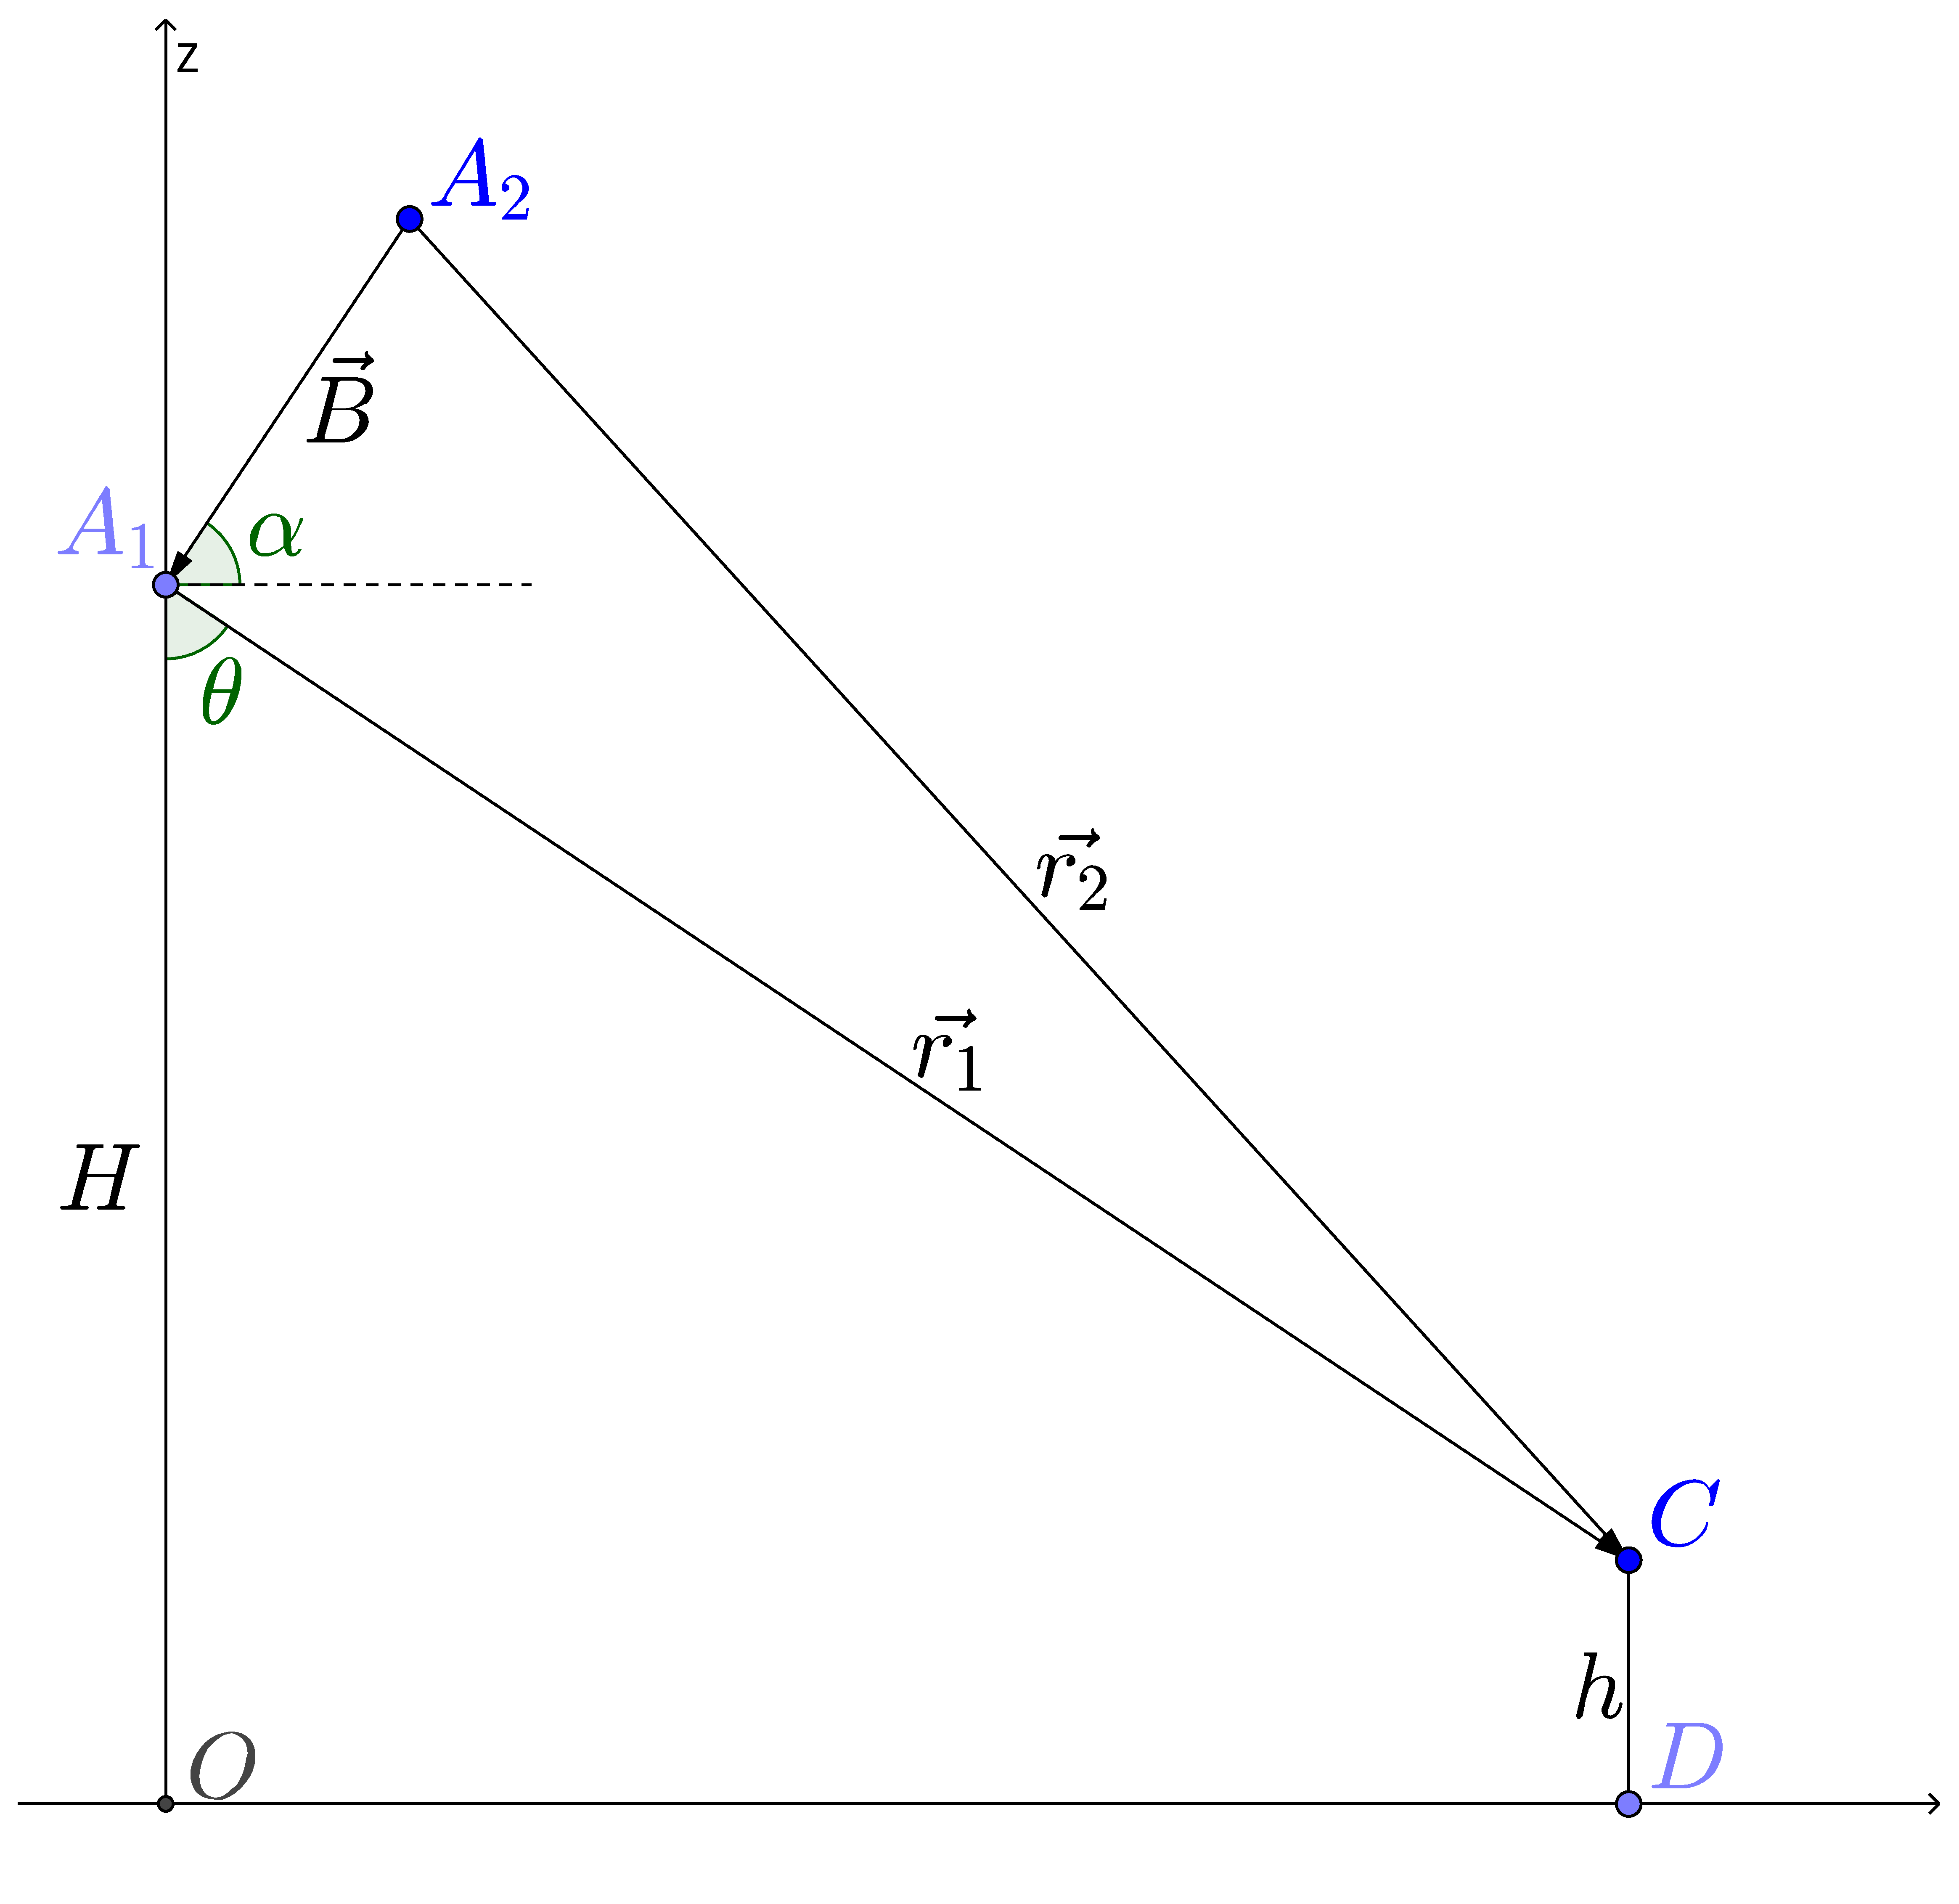
\includegraphics[width=0.6\textwidth]{figures/insar_simple.pdf}

            \resizebox{0.75\textwidth} {!} {
                \begin{minipage}{\linewidth}
                \begin{align*}
                    h &= H - r_1 \cos\theta \\
                    P_{\textrm{干涉}} &= P_1^* P_2 =  A_1 A_2 \exp(i \frac{4\pi}{\lambda}(r_2 - r_1)) \\
                    r_2 - r_1 &= r_1 \sqrt{1- \frac{\vec{r_1} \cdot \vec{B}}{r_1} + (\frac{B}{r_1})^2} \qquad \because B \ll |\vec{r}| \\
                              &\approx - \vec{r_1} \cdot \vec{B}
                              = - r_1 B \cos(\frac{\pi}{2} - \theta + \alpha)
                \end{align*}
                \end{minipage}
            }
        \end{column}
        \begin{column}{0.4\textwidth}
            \centering
            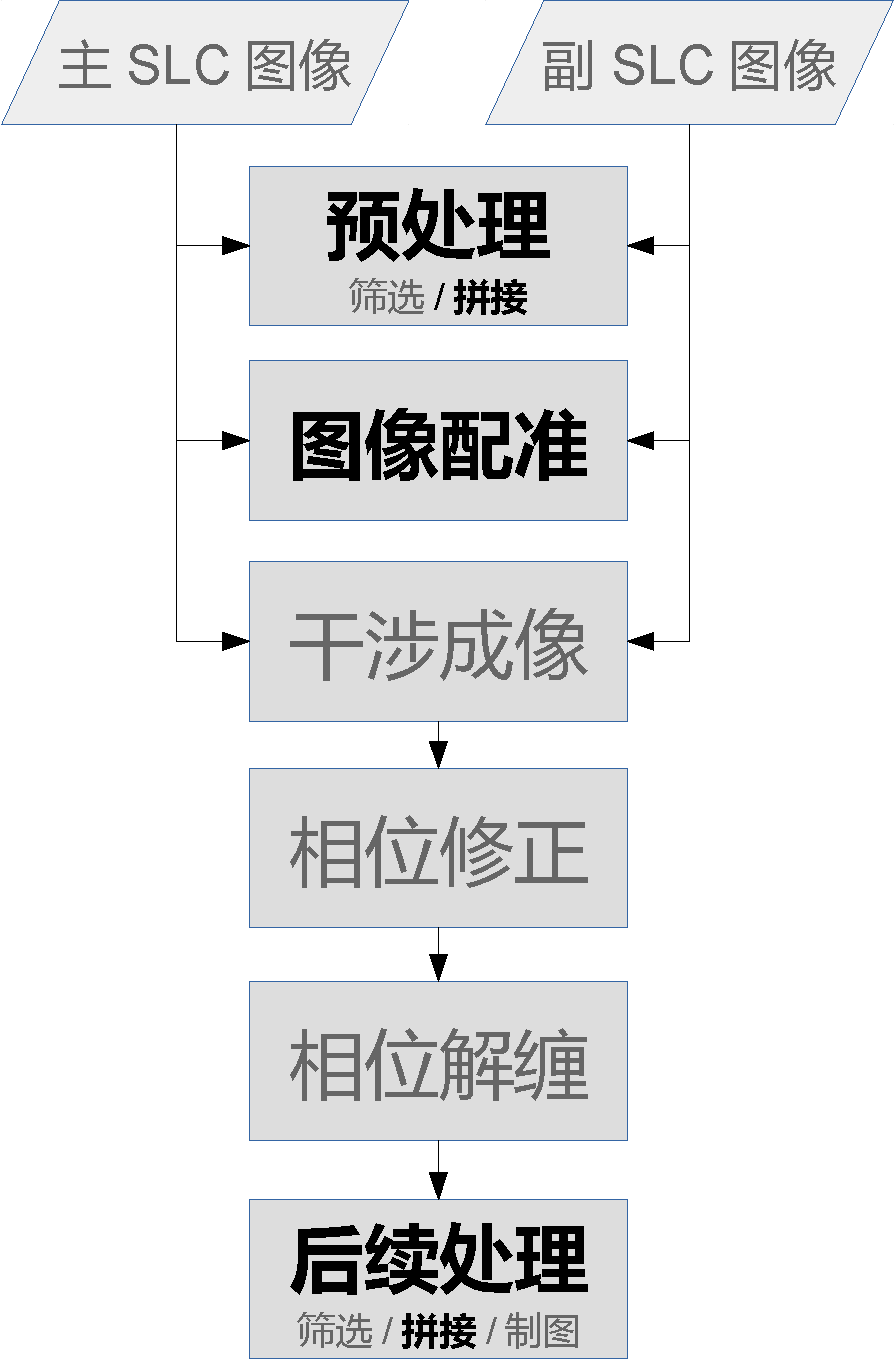
\includegraphics[width=0.8\textwidth]{figures/process.pdf}
        \end{column}
    \end{columns}
\end{frame}


\begin{frame}
    \frametitle{课题介绍}
    \framesubtitle{动机}

    InSAR 数据处理数据量大、计算复杂。\\~\\

    普通研究人员(我们)用桌面电脑处理数据:
    \begin{itemize}
        \setlength\itemsep{-0.1em}
        \item 软件串行处理,CPU 主频有限
        \item 完整流程等待 20min~hours
        \item 软件:GMTSAR(开源/免费)、ISCE(需要申请)
    \end{itemize}

    CPU 硬件发展:
    \begin{itemize}
        \setlength\itemsep{-0.1em}
        \item 主频达到瓶颈($<$4GHz)
        \item 多核心 CPU 普及 $\to$ 并行计算能力提升
    \end{itemize}

    要使用多核心 CPU 加速 InSAR 数据处理,必须将算法\textbf{并行化}。
\end{frame}

\begin{frame}
    \frametitle{课题介绍}
    \framesubtitle{成果}

    本课题:
    \begin{itemize}
        \item 以 GMTSAR 开源代码(串行算法)为范本
        \item 选取 InSAR 数据处理中两个模块,重写为并行程序:
        \begin{itemize}
            \item \textbf{图像配准}(image registration)
            \item \textbf{图像拼接}(image stitching)
        \end{itemize}
        \item 在实际 SAR 数据上测试了新程序,证明并行算法:
        \begin{itemize}
            \item 没有降低算法精度
            \item 大大提高了 InSAR 数据处理效率
        \end{itemize}
    \end{itemize}
\end{frame}


\begin{frame}
    \frametitle{算法设计}
    \framesubtitle{图像配准:GMTSAR xcorr}

    \begin{columns}
        \begin{column}{0.5\textwidth}
            \footnotesize
            \begin{center}
                图像配准 $(x_i, y_i) \to (x'_i, y'_i)$:
                \begin{equation*}
                    \begin{bmatrix}
                        t_i x_i' \\
                        t_i y_i' \\
                        t_i \\
                    \end{bmatrix}
                    = \begin{bmatrix}
                        a & b & c \\
                        d & e & f \\
                        0 & 0 & 1 \\
                    \end{bmatrix}
                    \begin{bmatrix}
                        x \\
                        y \\
                        1 \\
                    \end{bmatrix}
                \end{equation*}
                采样 $\to$ 局部配准 $\to$ 拟合全局参数\\
                要求精度:1/10 像素
            \end{center}

            局部配准:
            \begin{itemize}
                \item 粗配准(天线参数)+精配准\\
                \item \tiny $ (x'_c, y'_c)_{i,j} = (x_c, y_c)_{i,j} + (\Delta_x, \Delta_y) + (\delta_x, \delta_y)_{i,j} $
            \end{itemize}
        \end{column}
        \begin{column}{0.5\textwidth}
            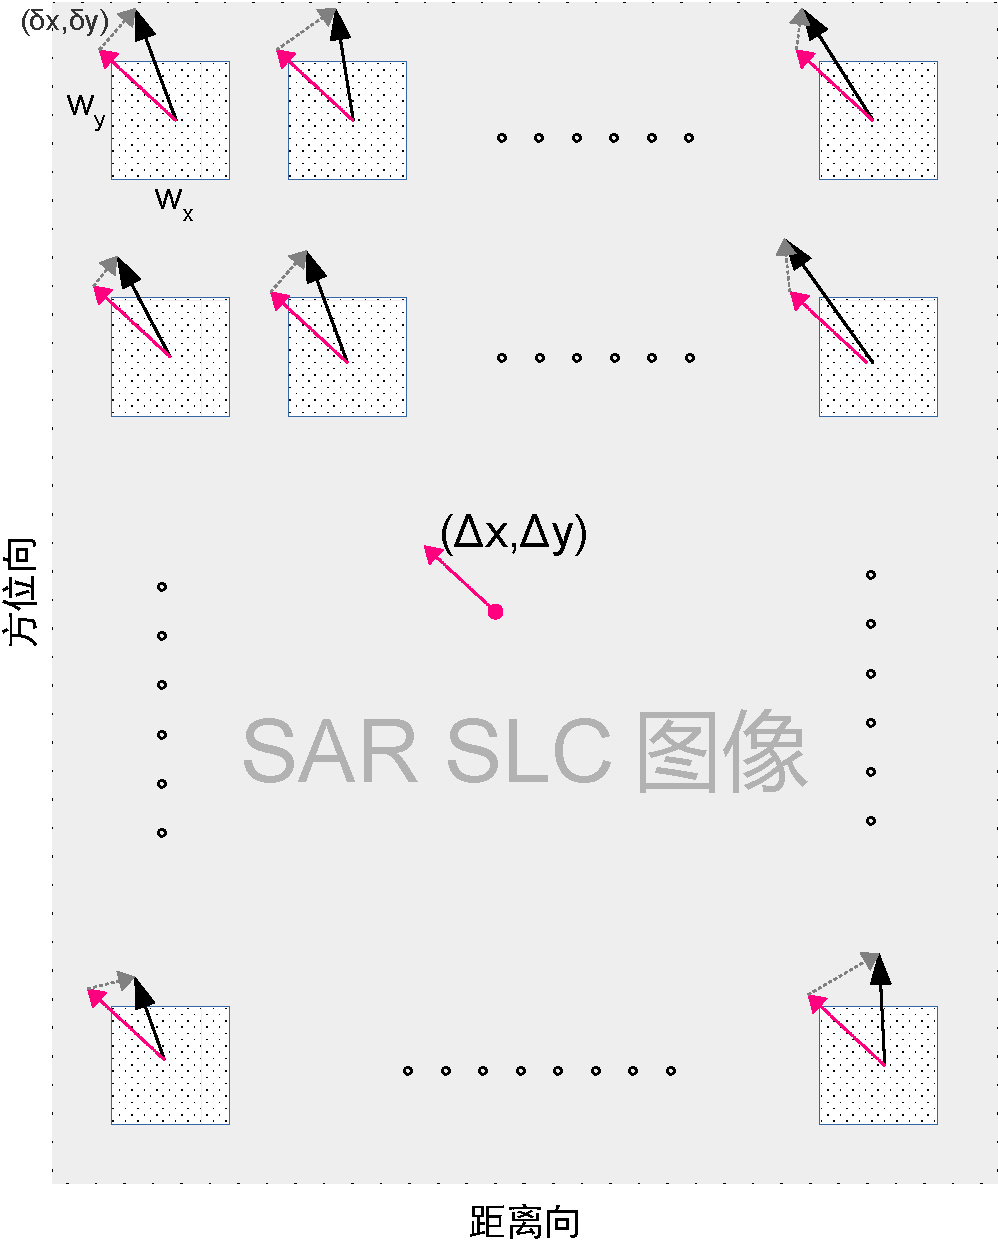
\includegraphics[width=0.80\textwidth]{figures/register.pdf}
        \end{column}
    \end{columns}

    \centering
    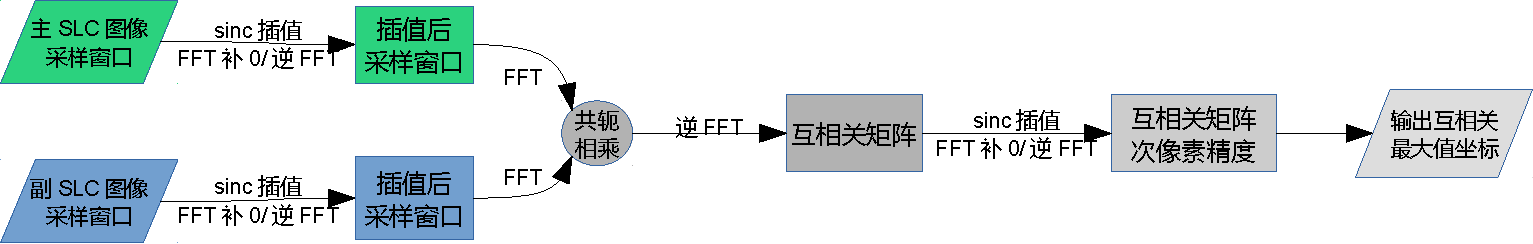
\includegraphics[width=0.99\textwidth]{figures/xcorr-crop.pdf}
\end{frame}

\begin{frame}
    \frametitle{算法设计}
    \framesubtitle{图像配准优化:xcorr2}

    \begin{block}{简化 FFT}
        局部配准只用到复像素的幅值(散射系数幅度):
        \begin{itemize}
            \item GMTSAR xcorr:9 次 FFT(或逆变换)
            \item xcorr2:4 次 FFT + 5 次实序列 FFT
        \end{itemize}
        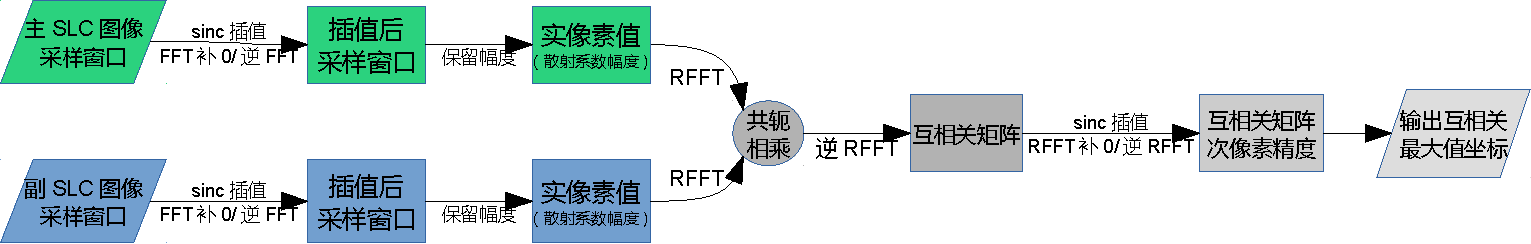
\includegraphics[width=0.99\textwidth]{figures/xcorr2-crop.pdf}
    \end{block}
\end{frame}



\begin{frame}
    \frametitle{算法设计}
    \framesubtitle{图像配准优化:xcorr2}

    \begin{columns}
        \begin{column}{0.5\textwidth}
            \begin{block}{主-副多线程架构}
            \begin{itemize}
                \item 主线程加载采样窗口图像
                \begin{itemize}
                    \item 预读取
                    \item 启动计算线程
                \end{itemize}
                \item 计算线程执行局部配准
            \end{itemize}
            \end{block}

            \begin{block}{特点}
            \begin{itemize}
                \item 任务分割粒度小 \\ \begin{scriptsize} 512 采样窗口 vs 4~16 核心 \end{scriptsize}
                \item 数据量大,避免竞争 IO \\ \begin{scriptsize} 磁盘顺序读写优势 \end{scriptsize}
            \end{itemize}
            \end{block}
        \end{column}
        \begin{column}{0.5\textwidth}
            \centering
            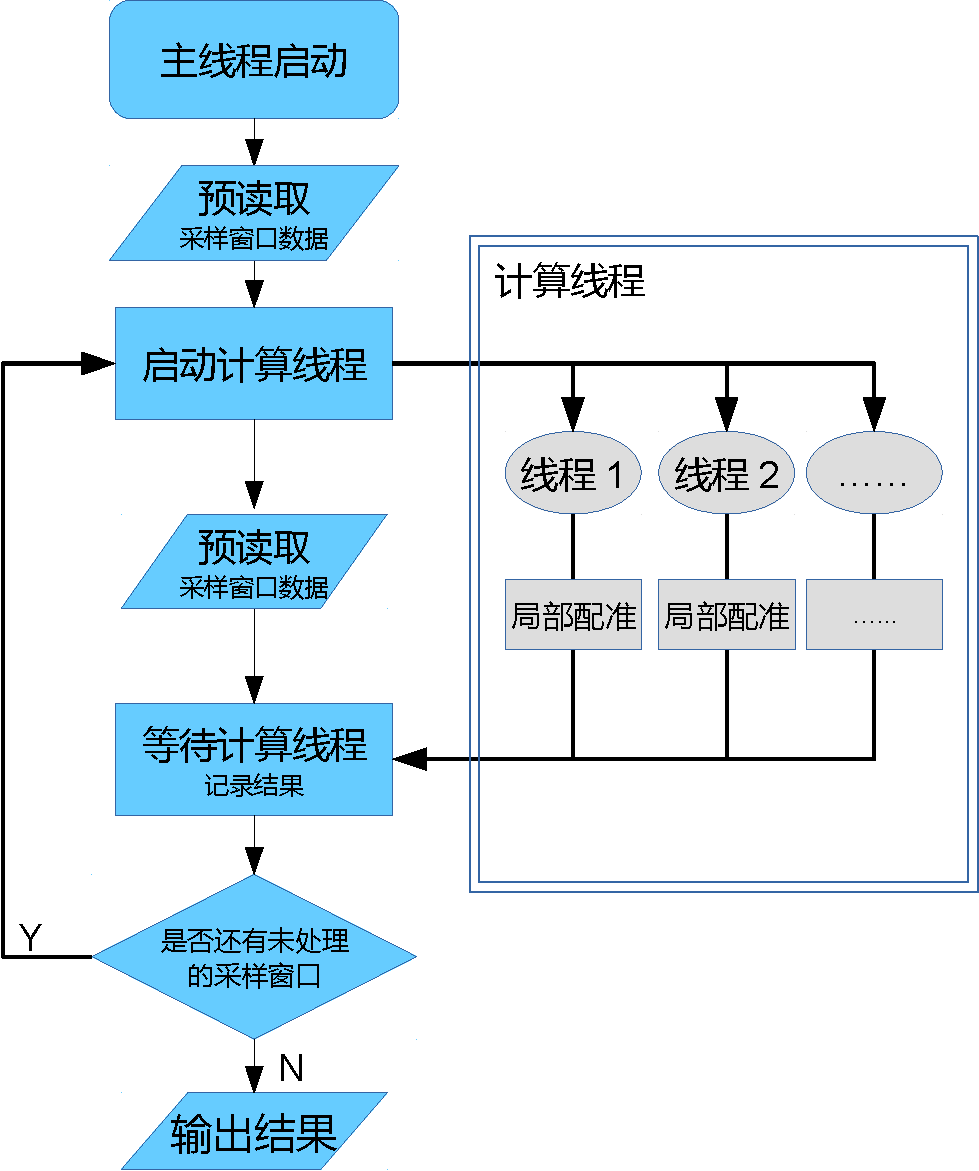
\includegraphics[width=0.99\textwidth]{figures/parallel.pdf}
        \end{column}
    \end{columns}
\end{frame}


\begin{frame}
    \frametitle{算法设计}
    \framesubtitle{图像拼接}

    \begin{columns}
        \begin{column}{0.5\textwidth}
            \begin{block}{应用}
                \small
                得到大范围的 InSAR 图像
                \begin{itemize}
                    \item 预处理:拼接 SAR 数据
                    \item InSAR 成像后:拼接干涉图
                \end{itemize}
            \end{block}
            \begin{block}{特点/困难}
                \small
                \begin{itemize}
                    \item 多个输入 $\to$ 单一输出
                    \item 必须保持拼接顺序
                \end{itemize}
            \end{block}
        \end{column}
        \begin{column}{0.5\textwidth}
            \centering
            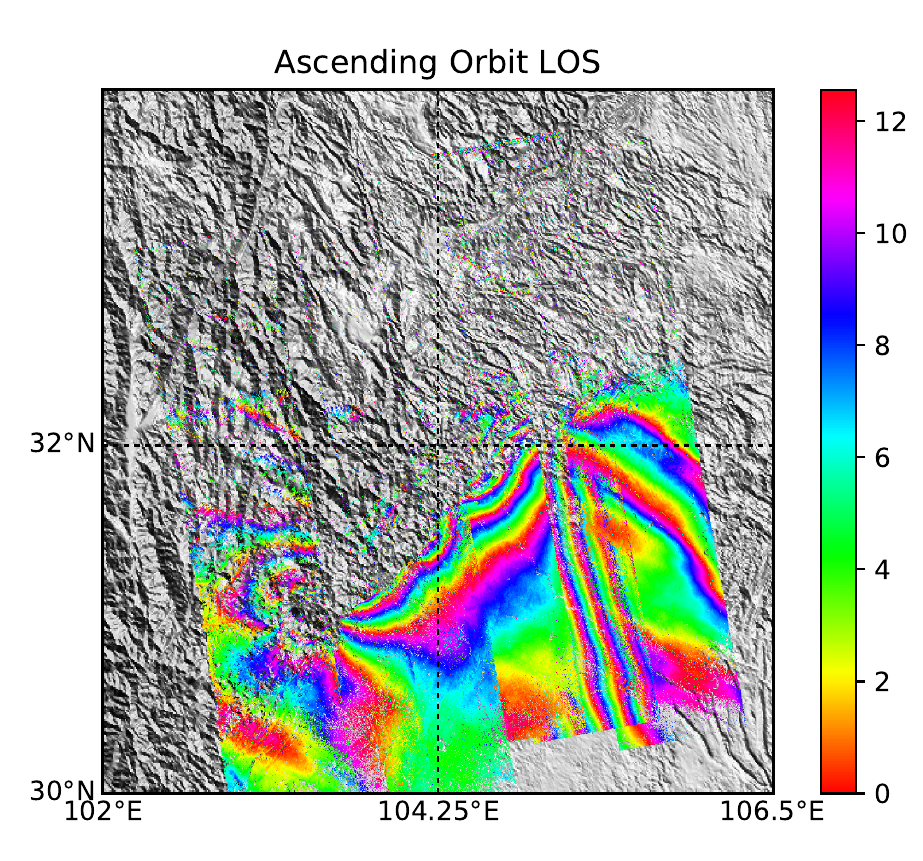
\includegraphics[width=0.99\textwidth]{figures/wenchuan.png}
            \begin{tiny}
            *反映汶川地震前后地表形变的 InSAR 图像 \\
            (地空学院金泽宇同学提供)
            \end{tiny}
        \end{column}
    \end{columns}
\end{frame}


\begin{frame}
    \frametitle{算法设计}
    \framesubtitle{图像拼接优化}

    \begin{columns}
        \begin{column}{0.5\textwidth}
            \begin{block}{归约技术(reduce)}
                \small
                可结合/不可交换运算的并行化
                \begin{itemize}
                    \item 分组拼接相邻文件
                    \item 多轮迭代至完成
                \end{itemize}
                计算任务不平衡(收敛到单线程)
            \end{block}
        \end{column}
        \begin{column}{0.5\textwidth}
            \centering
            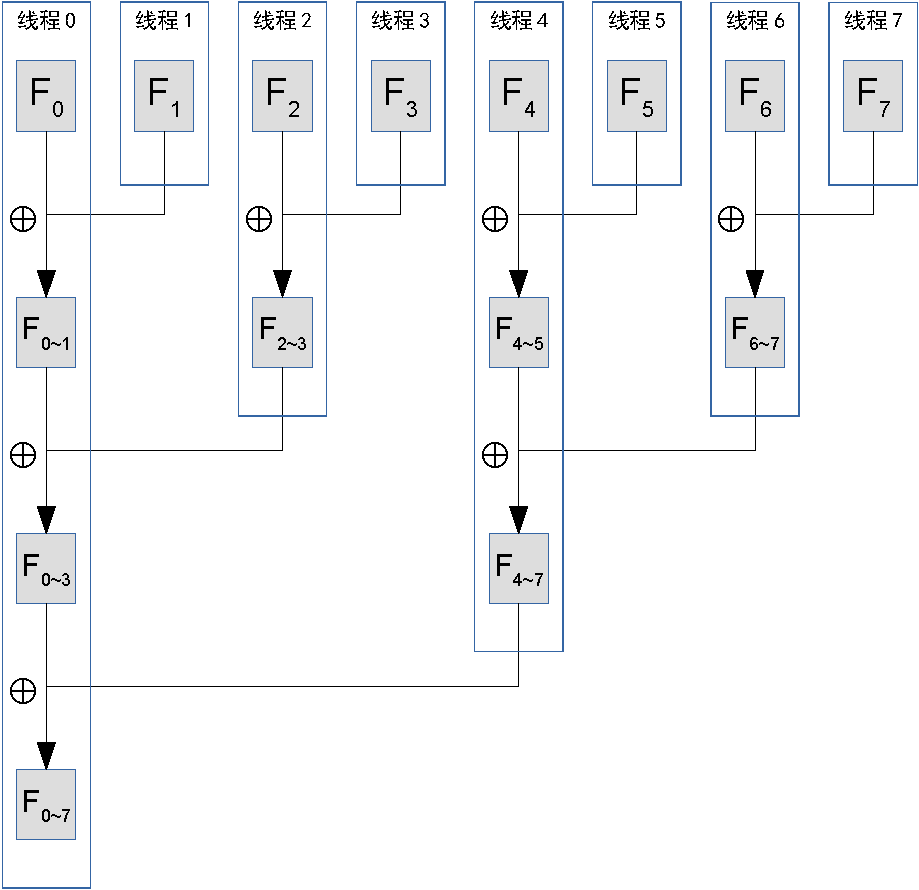
\includegraphics[width=0.99\textwidth]{figures/reduce.pdf}
            \begin{tiny}
            8个文件的并行归约拼接示意图
            \end{tiny}
        \end{column}
    \end{columns}
\end{frame}


\begin{frame}
    \frametitle{实验评估}
    \framesubtitle{环境}

    \begin{block}{实验环境}
        \small
        \begin{itemize}
            \setlength\itemsep{-0.1em}
            \item Intel Xeon E5-2650 v4 @2.20GHz (12核)
            \item Ubuntu 16.04.2
            \item gcc 5.4.0 (-O2 优化)
        \end{itemize}
    \end{block}
 
    \begin{block}{实验数据}
        \small
        \begin{itemize}
            \setlength\itemsep{-0.1em}
            \item 2010 Baja Earthquake ($7.2 M_w$)
            \item ALOS 卫星数据(下载自 GMTSAR 网站)
        \end{itemize}
    \end{block}
\end{frame}


\begin{frame}
    \frametitle{实验评估}
    \framesubtitle{图像拼接}

    6 帧 SAR 图像拼接效率 \\~\\
    \begin{columns}
        \begin{column}{0.5\textwidth}
            \centering
            \resizebox {\textwidth} {!} {
                \begin{tikzpicture}
\begin{axis}[
    xlabel={并行线程数},
    ylabel={计算时间/s},
    xmin=1, xmax=7,
    ymin=0, ymax=200,
    xtick={1, 2, 3, 4, 5, 6, 7},
%    ytick={ },
    legend pos=north east,
    ymajorgrids=true,
    grid style=dashed,
]

\addplot[
    color=red,
    mark=square,
    style=solid,
    ]
    coordinates {
        (1, 194.972254756)
        (2, 106.441216719)
        (3, 91.799094679)
        (4, 92.142388643)
        (5, 92.000214744)
        (6, 88.829891908)
        (7, 83.641275544)
    };
\end{axis}
\end{tikzpicture}

            }
        \end{column}
        \begin{column}{0.5\textwidth}
            \centering
            \resizebox {\textwidth} {!} {
                \begin{tikzpicture}
\begin{axis}[
    xlabel={并行线程数},
    ylabel={CPU 核心占用},
    xmin=1, xmax=7,
    ymin=0, ymax=4,
    xtick={1, 2, 3, 4, 5, 6, 7},
%    ytick={ },
    legend pos=north east,
    ymajorgrids=true,
    grid style=dashed,
]

\addplot[
    color=red,
    mark=square,
    style=solid,
    ]
    coordinates {
        (1, 1.000)
        (2, 1.862)
        (3, 2.257)
        (4, 2.258)
        (5, 2.298)
        (6, 2.425)
        (7, 2.575)
    };
\end{axis}
\end{tikzpicture}

            }
        \end{column}
    \end{columns}

    \begin{itemize}
        \small
        \setlength\itemsep{-0.1em}
        \item 数据太少,收敛太快
        \item 仍然节省了一半的时间
    \end{itemize}
\end{frame}


\begin{frame}
    \frametitle{实验评估}
    \framesubtitle{图像配准}

    SLC 图像配准效率 \\~\\
    \begin{columns}
        \begin{column}{0.5\textwidth}
            \centering
            \resizebox {\textwidth} {!} {
                \begin{tikzpicture}
\begin{semilogyaxis}[
    xlabel={采样窗口数量},
    ylabel={计算时间/s},
    xmin=0, xmax=5000,
    ymin=0.5, ymax=250,
    ytick={0.5, 1, 2, 5, 10, 20, 50, 100, 200 },
    legend style={at={(0.97,0.16)},anchor=east,font=\small},
    ymajorgrids=true,
    grid style=dashed,
    log ticks with fixed point,
]

\addplot[
    color=blue,
    mark=triangle*,
    style=densely dashed,
    ]
    coordinates {
        (4608, 229.347642791)
        (3200, 157.700291651)
        (2048, 96.024747129)
        (1152, 51.340117550)
        (512, 21.212574205)
        (128, 5.638659853)
    };
    \addlegendentry{GMTSAR xcorr}

\addplot[
    color=red,
    mark=diamond*,
    style=densely dotted,
    ]
    coordinates {
        (4608, 25.681487185)
        (3200, 19.249105679)
        (2048, 12.470892872)
        (1152, 7.826916179)
        (512, 4.082934246)
        (128, 1.411728191)
    };
    \addlegendentry{xcorr2(单线程)}

\addplot[
    color=brown,
    mark=square*,
    style=solid,
    ]
    coordinates {
        (4608, 7.579960118)
        (3200, 5.624775143)
        (2048, 4.246431781)
        (1152, 3.118109658)
        (512, 1.859684801)
        (128, 0.914280470)
    };
    \addlegendentry{xcorr2(8线程)}

\end{semilogyaxis}
\end{tikzpicture}

            }
        \end{column}
        \begin{column}{0.5\textwidth}
            \centering
            \resizebox {\textwidth} {!} {
                \begin{tikzpicture}
\begin{axis}[
    xlabel={采样窗口数量},
    ylabel={占用 CPU 核心数},
    xmin=0, xmax=5000,
    ymin=0, ymax=6,
    ytick={ 0, 1, 2, 3, 4, 5, 6 },
    legend style={at={(0.97,0.7)},anchor=east,font=\small},
    ymajorgrids=true,
    grid style=dashed,
]

\addplot[
    color=blue,
    mark=triangle*,
    style=densely dashed,
    ]
    coordinates {
        (4608, 2.589)
        (3200, 2.520)
        (2048, 2.439)
        (1152, 2.074)
        (512, 2.108)
        (128, 2.118)
    };
    \addlegendentry{GMTSAR xcorr}

\addplot[
    color=red,
    mark=diamond*,
    style=densely dotted,
    ]
    coordinates {
        (4608, 1.000)
        (3200, 1.000)
        (2048, 1.000)
        (1152, 1.000)
        (512, 1.000)
        (128, 0.999)
    };
    \addlegendentry{xcorr2(单线程)}

\addplot[
    color=brown,
    mark=square*,
    style=solid,
    ]
    coordinates {
        (4608, 5.899)
        (3200, 5.674)
        (2048, 5.283)
        (1152, 4.705)
        (512, 3.906)
        (128, 2.621)
    };
    \addlegendentry{xcorr2(8线程)}

\end{axis}
\end{tikzpicture}

            }
        \end{column}
    \end{columns}

    \begin{itemize}
        \small
        \setlength\itemsep{-0.1em}
        \item 单线程就有了很大提升:FFT 优化、编译器优化?
        \item 并行算法加速 6~30 倍!
    \end{itemize}
\end{frame}

\begin{frame}
    \frametitle{实验评估}
    \framesubtitle{图像配准}

    精配准偏移比较(仅显示矢量长度) \\~\\
    \begin{columns}
        \begin{column}{0.3\textwidth}
            \centering
            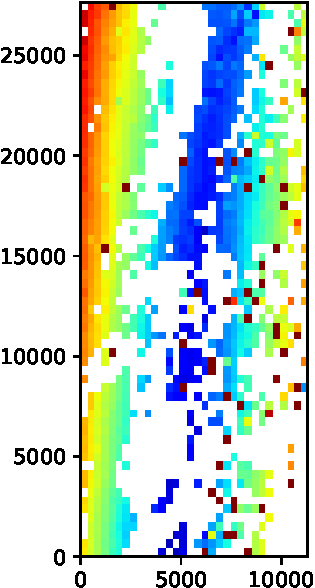
\includegraphics[width=0.8\textwidth]{figures/xcorr-result}\\
            \begin{scriptsize} GMTSAR xcorr \end{scriptsize}
        \end{column}
        \begin{column}{0.3\textwidth}
            \centering
            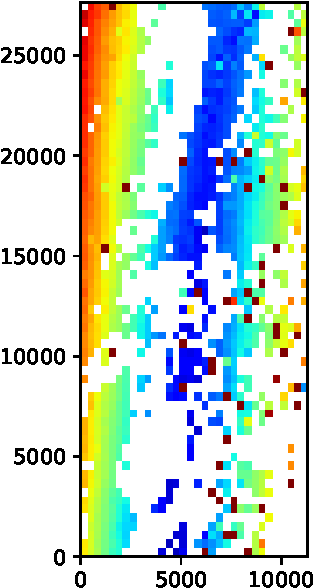
\includegraphics[width=0.8\textwidth]{figures/xcorr2-result}\\
            \begin{scriptsize} xcorr2 \end{scriptsize}
        \end{column}
        \begin{column}{0.39\textwidth}
            \centering
            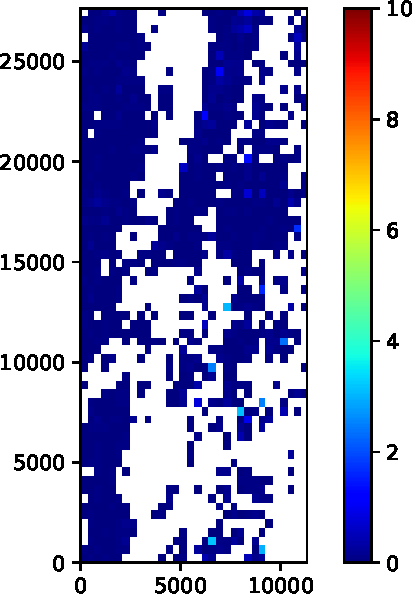
\includegraphics[width=0.8\textwidth]{figures/diff-result}\\
            \begin{scriptsize} 矢量差 \end{scriptsize}
        \end{column}
    \end{columns}

    ~\\
    98.8\% 有效配准结果差异不超过1个像素
\end{frame}


\begin{frame}
    \frametitle{实验评估}
    \framesubtitle{图像配准}

    相干性:
    \resizebox{0.7\textwidth} {!} {
        \begin{minipage}{\linewidth}
            \begin{equation*}
                \gamma(x, y) = \frac{\sum_{x', y'} P_1(x', y') P_2^*(x', y')}{\sqrt{\sum_{x', y'}|P_1(x', y')|^2 \sum_{x', y'}|P_2(x', y')|^2}} \qquad (x', y') \in D(x, y)
            \end{equation*}
        \end{minipage}
    }
    \\~\\
    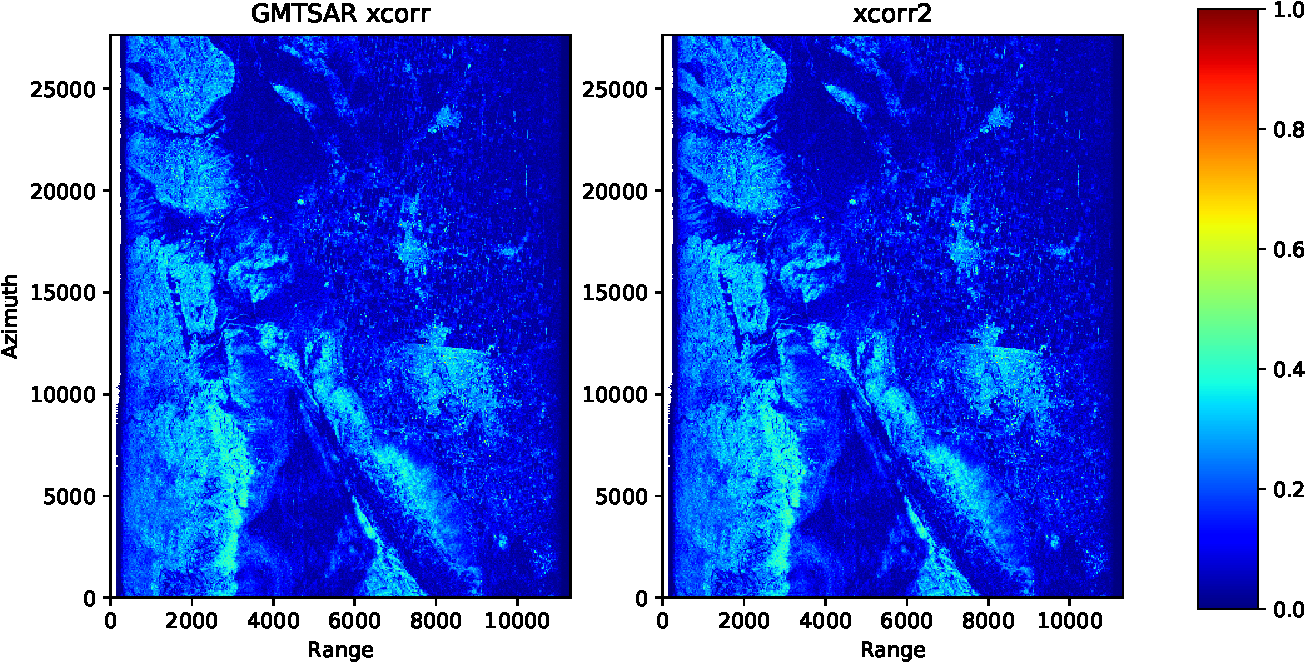
\includegraphics[width=0.99\textwidth]{figures/coh-two}
\end{frame}

\begin{frame}
    \frametitle{实验评估}
    \framesubtitle{图像配准}

    相干性差异 < 0.003 \\
    \centering
    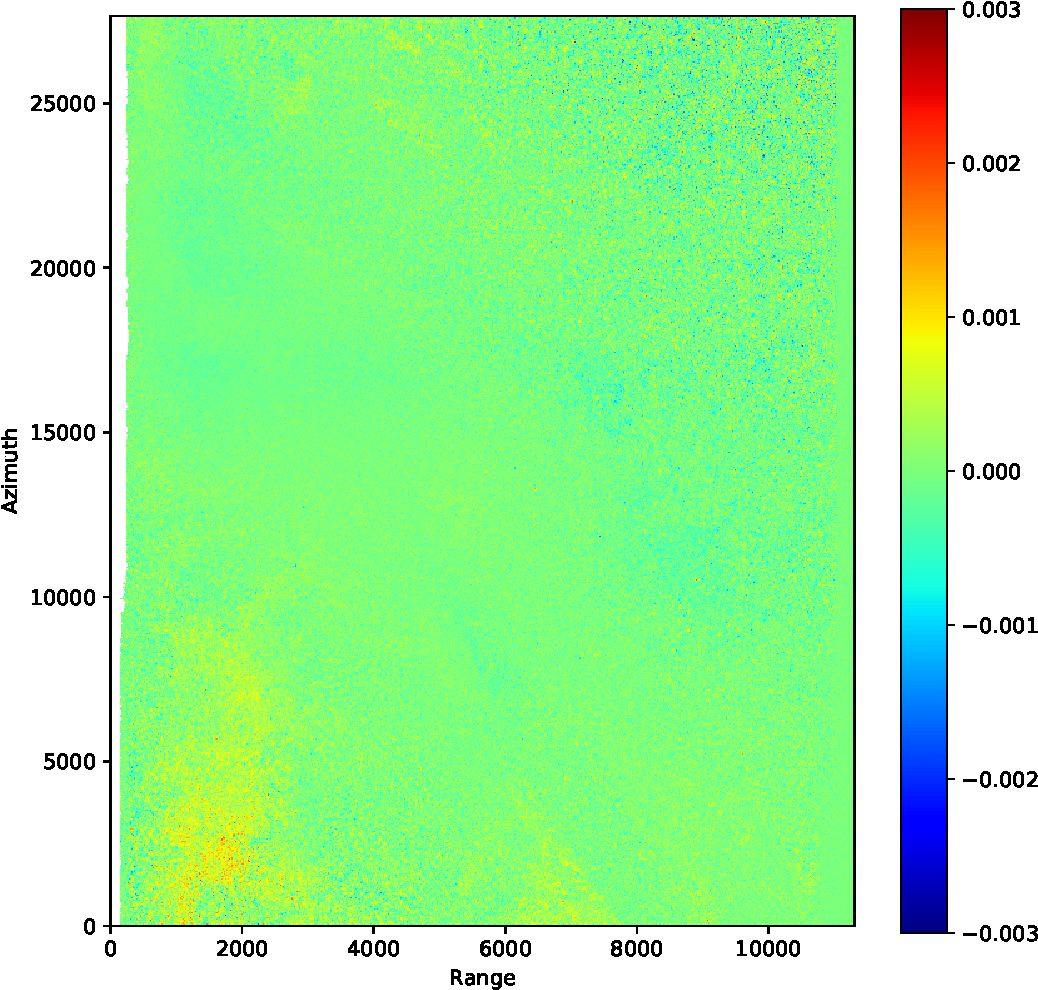
\includegraphics[width=0.6\textwidth]{figures/coh-diff}
    ~\\
    \begin{scriptsize} 用上页 xcorr2 的结果减去 GMTSAR xcorr 的结果 \end{scriptsize}
\end{frame}


\begin{frame}
    \frametitle{其他贡献}

    提交了三项 GMTSAR 软件问题:
    \begin{scriptsize} \url{http://gmt.soest.hawaii.edu/projects/gmt5sar/issues} \end{scriptsize}\\
    一个问题已经被夏威夷大学开发者 Paul Wessel 修复 \\~\\

    \centering
    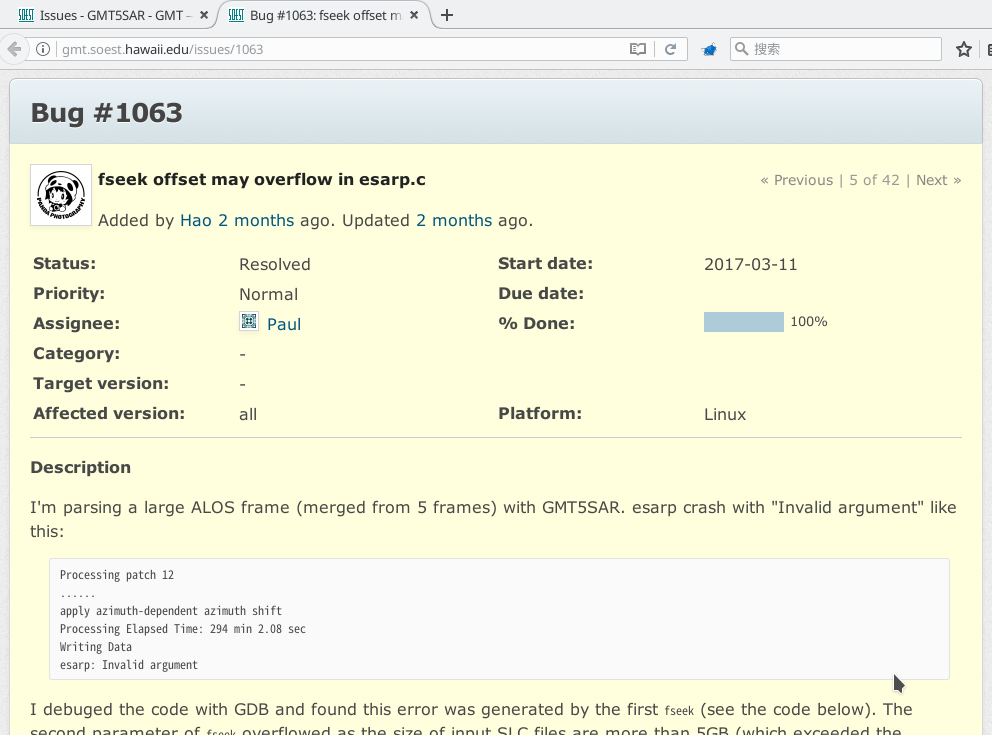
\includegraphics[width=0.85\textwidth,trim={0 5cm 0 0},clip]{figures/issue.png}
\end{frame}


\begin{frame}
    \frametitle{附录}

    \begin{itemize}
        \item 本课题全部代码发布在\\ \url{https://github.com/cuihaoleo/gmtsar_optimize}
        \item 所有图表未注明引用的均为自制
        \item 主要参考文献:\\
        \begin{itemize}
            \scriptsize
            \item[] Simons M, Rosen P A. Interferometric synthetic aperture radar geodesy[J]. 2007.
            \item[] Sandwell D, Mellors R, Tong X, et al. Gmtsar: An insar processing system based on generic mapping tools[J]. Scripps Institution of Oceanography, 2011.
            \item[] Ferretti A, Monti-Guarnieri A, Prati C, et al. InSAR principles-guidelines for SAR interferometry processing and interpretation[M]. 2007.
        \end{itemize}
    \end{itemize}
\end{frame}

\end{document}
